
% Default to the notebook output style

    


% Inherit from the specified cell style.




    
\documentclass[11pt]{article}

    
    
    \usepackage[T1]{fontenc}
    % Nicer default font (+ math font) than Computer Modern for most use cases
    \usepackage{mathpazo}

    % Basic figure setup, for now with no caption control since it's done
    % automatically by Pandoc (which extracts ![](path) syntax from Markdown).
    \usepackage{graphicx}
    % We will generate all images so they have a width \maxwidth. This means
    % that they will get their normal width if they fit onto the page, but
    % are scaled down if they would overflow the margins.
    \makeatletter
    \def\maxwidth{\ifdim\Gin@nat@width>\linewidth\linewidth
    \else\Gin@nat@width\fi}
    \makeatother
    \let\Oldincludegraphics\includegraphics
    % Set max figure width to be 80% of text width, for now hardcoded.
    \renewcommand{\includegraphics}[1]{\Oldincludegraphics[width=.8\maxwidth]{#1}}
    % Ensure that by default, figures have no caption (until we provide a
    % proper Figure object with a Caption API and a way to capture that
    % in the conversion process - todo).
    \usepackage{caption}
    \DeclareCaptionLabelFormat{nolabel}{}
    \captionsetup{labelformat=nolabel}

    \usepackage{adjustbox} % Used to constrain images to a maximum size 
    \usepackage{xcolor} % Allow colors to be defined
    \usepackage{enumerate} % Needed for markdown enumerations to work
    \usepackage{geometry} % Used to adjust the document margins
    \usepackage{amsmath} % Equations
    \usepackage{amssymb} % Equations
    \usepackage{textcomp} % defines textquotesingle
    % Hack from http://tex.stackexchange.com/a/47451/13684:
    \AtBeginDocument{%
        \def\PYZsq{\textquotesingle}% Upright quotes in Pygmentized code
    }
    \usepackage{upquote} % Upright quotes for verbatim code
    \usepackage{eurosym} % defines \euro
    \usepackage[mathletters]{ucs} % Extended unicode (utf-8) support
    \usepackage[utf8x]{inputenc} % Allow utf-8 characters in the tex document
    \usepackage{fancyvrb} % verbatim replacement that allows latex
    \usepackage{grffile} % extends the file name processing of package graphics 
                         % to support a larger range 
    % The hyperref package gives us a pdf with properly built
    % internal navigation ('pdf bookmarks' for the table of contents,
    % internal cross-reference links, web links for URLs, etc.)
    \usepackage{hyperref}
    \usepackage{longtable} % longtable support required by pandoc >1.10
    \usepackage{booktabs}  % table support for pandoc > 1.12.2
    \usepackage[inline]{enumitem} % IRkernel/repr support (it uses the enumerate* environment)
    \usepackage[normalem]{ulem} % ulem is needed to support strikethroughs (\sout)
                                % normalem makes italics be italics, not underlines
    

    
    
    % Colors for the hyperref package
    \definecolor{urlcolor}{rgb}{0,.145,.698}
    \definecolor{linkcolor}{rgb}{.71,0.21,0.01}
    \definecolor{citecolor}{rgb}{.12,.54,.11}

    % ANSI colors
    \definecolor{ansi-black}{HTML}{3E424D}
    \definecolor{ansi-black-intense}{HTML}{282C36}
    \definecolor{ansi-red}{HTML}{E75C58}
    \definecolor{ansi-red-intense}{HTML}{B22B31}
    \definecolor{ansi-green}{HTML}{00A250}
    \definecolor{ansi-green-intense}{HTML}{007427}
    \definecolor{ansi-yellow}{HTML}{DDB62B}
    \definecolor{ansi-yellow-intense}{HTML}{B27D12}
    \definecolor{ansi-blue}{HTML}{208FFB}
    \definecolor{ansi-blue-intense}{HTML}{0065CA}
    \definecolor{ansi-magenta}{HTML}{D160C4}
    \definecolor{ansi-magenta-intense}{HTML}{A03196}
    \definecolor{ansi-cyan}{HTML}{60C6C8}
    \definecolor{ansi-cyan-intense}{HTML}{258F8F}
    \definecolor{ansi-white}{HTML}{C5C1B4}
    \definecolor{ansi-white-intense}{HTML}{A1A6B2}

    % commands and environments needed by pandoc snippets
    % extracted from the output of `pandoc -s`
    \providecommand{\tightlist}{%
      \setlength{\itemsep}{0pt}\setlength{\parskip}{0pt}}
    \DefineVerbatimEnvironment{Highlighting}{Verbatim}{commandchars=\\\{\}}
    % Add ',fontsize=\small' for more characters per line
    \newenvironment{Shaded}{}{}
    \newcommand{\KeywordTok}[1]{\textcolor[rgb]{0.00,0.44,0.13}{\textbf{{#1}}}}
    \newcommand{\DataTypeTok}[1]{\textcolor[rgb]{0.56,0.13,0.00}{{#1}}}
    \newcommand{\DecValTok}[1]{\textcolor[rgb]{0.25,0.63,0.44}{{#1}}}
    \newcommand{\BaseNTok}[1]{\textcolor[rgb]{0.25,0.63,0.44}{{#1}}}
    \newcommand{\FloatTok}[1]{\textcolor[rgb]{0.25,0.63,0.44}{{#1}}}
    \newcommand{\CharTok}[1]{\textcolor[rgb]{0.25,0.44,0.63}{{#1}}}
    \newcommand{\StringTok}[1]{\textcolor[rgb]{0.25,0.44,0.63}{{#1}}}
    \newcommand{\CommentTok}[1]{\textcolor[rgb]{0.38,0.63,0.69}{\textit{{#1}}}}
    \newcommand{\OtherTok}[1]{\textcolor[rgb]{0.00,0.44,0.13}{{#1}}}
    \newcommand{\AlertTok}[1]{\textcolor[rgb]{1.00,0.00,0.00}{\textbf{{#1}}}}
    \newcommand{\FunctionTok}[1]{\textcolor[rgb]{0.02,0.16,0.49}{{#1}}}
    \newcommand{\RegionMarkerTok}[1]{{#1}}
    \newcommand{\ErrorTok}[1]{\textcolor[rgb]{1.00,0.00,0.00}{\textbf{{#1}}}}
    \newcommand{\NormalTok}[1]{{#1}}
    
    % Additional commands for more recent versions of Pandoc
    \newcommand{\ConstantTok}[1]{\textcolor[rgb]{0.53,0.00,0.00}{{#1}}}
    \newcommand{\SpecialCharTok}[1]{\textcolor[rgb]{0.25,0.44,0.63}{{#1}}}
    \newcommand{\VerbatimStringTok}[1]{\textcolor[rgb]{0.25,0.44,0.63}{{#1}}}
    \newcommand{\SpecialStringTok}[1]{\textcolor[rgb]{0.73,0.40,0.53}{{#1}}}
    \newcommand{\ImportTok}[1]{{#1}}
    \newcommand{\DocumentationTok}[1]{\textcolor[rgb]{0.73,0.13,0.13}{\textit{{#1}}}}
    \newcommand{\AnnotationTok}[1]{\textcolor[rgb]{0.38,0.63,0.69}{\textbf{\textit{{#1}}}}}
    \newcommand{\CommentVarTok}[1]{\textcolor[rgb]{0.38,0.63,0.69}{\textbf{\textit{{#1}}}}}
    \newcommand{\VariableTok}[1]{\textcolor[rgb]{0.10,0.09,0.49}{{#1}}}
    \newcommand{\ControlFlowTok}[1]{\textcolor[rgb]{0.00,0.44,0.13}{\textbf{{#1}}}}
    \newcommand{\OperatorTok}[1]{\textcolor[rgb]{0.40,0.40,0.40}{{#1}}}
    \newcommand{\BuiltInTok}[1]{{#1}}
    \newcommand{\ExtensionTok}[1]{{#1}}
    \newcommand{\PreprocessorTok}[1]{\textcolor[rgb]{0.74,0.48,0.00}{{#1}}}
    \newcommand{\AttributeTok}[1]{\textcolor[rgb]{0.49,0.56,0.16}{{#1}}}
    \newcommand{\InformationTok}[1]{\textcolor[rgb]{0.38,0.63,0.69}{\textbf{\textit{{#1}}}}}
    \newcommand{\WarningTok}[1]{\textcolor[rgb]{0.38,0.63,0.69}{\textbf{\textit{{#1}}}}}
    
    
    % Define a nice break command that doesn't care if a line doesn't already
    % exist.
    \def\br{\hspace*{\fill} \\* }
    % Math Jax compatability definitions
    \def\gt{>}
    \def\lt{<}
    % Document parameters
    \title{home\_credit\_default\_risk}
    
    
    

    % Pygments definitions
    
\makeatletter
\def\PY@reset{\let\PY@it=\relax \let\PY@bf=\relax%
    \let\PY@ul=\relax \let\PY@tc=\relax%
    \let\PY@bc=\relax \let\PY@ff=\relax}
\def\PY@tok#1{\csname PY@tok@#1\endcsname}
\def\PY@toks#1+{\ifx\relax#1\empty\else%
    \PY@tok{#1}\expandafter\PY@toks\fi}
\def\PY@do#1{\PY@bc{\PY@tc{\PY@ul{%
    \PY@it{\PY@bf{\PY@ff{#1}}}}}}}
\def\PY#1#2{\PY@reset\PY@toks#1+\relax+\PY@do{#2}}

\expandafter\def\csname PY@tok@cs\endcsname{\let\PY@it=\textit\def\PY@tc##1{\textcolor[rgb]{0.25,0.50,0.50}{##1}}}
\expandafter\def\csname PY@tok@c1\endcsname{\let\PY@it=\textit\def\PY@tc##1{\textcolor[rgb]{0.25,0.50,0.50}{##1}}}
\expandafter\def\csname PY@tok@si\endcsname{\let\PY@bf=\textbf\def\PY@tc##1{\textcolor[rgb]{0.73,0.40,0.53}{##1}}}
\expandafter\def\csname PY@tok@sa\endcsname{\def\PY@tc##1{\textcolor[rgb]{0.73,0.13,0.13}{##1}}}
\expandafter\def\csname PY@tok@vg\endcsname{\def\PY@tc##1{\textcolor[rgb]{0.10,0.09,0.49}{##1}}}
\expandafter\def\csname PY@tok@mf\endcsname{\def\PY@tc##1{\textcolor[rgb]{0.40,0.40,0.40}{##1}}}
\expandafter\def\csname PY@tok@mh\endcsname{\def\PY@tc##1{\textcolor[rgb]{0.40,0.40,0.40}{##1}}}
\expandafter\def\csname PY@tok@kd\endcsname{\let\PY@bf=\textbf\def\PY@tc##1{\textcolor[rgb]{0.00,0.50,0.00}{##1}}}
\expandafter\def\csname PY@tok@sc\endcsname{\def\PY@tc##1{\textcolor[rgb]{0.73,0.13,0.13}{##1}}}
\expandafter\def\csname PY@tok@nd\endcsname{\def\PY@tc##1{\textcolor[rgb]{0.67,0.13,1.00}{##1}}}
\expandafter\def\csname PY@tok@nv\endcsname{\def\PY@tc##1{\textcolor[rgb]{0.10,0.09,0.49}{##1}}}
\expandafter\def\csname PY@tok@m\endcsname{\def\PY@tc##1{\textcolor[rgb]{0.40,0.40,0.40}{##1}}}
\expandafter\def\csname PY@tok@w\endcsname{\def\PY@tc##1{\textcolor[rgb]{0.73,0.73,0.73}{##1}}}
\expandafter\def\csname PY@tok@vi\endcsname{\def\PY@tc##1{\textcolor[rgb]{0.10,0.09,0.49}{##1}}}
\expandafter\def\csname PY@tok@cm\endcsname{\let\PY@it=\textit\def\PY@tc##1{\textcolor[rgb]{0.25,0.50,0.50}{##1}}}
\expandafter\def\csname PY@tok@s\endcsname{\def\PY@tc##1{\textcolor[rgb]{0.73,0.13,0.13}{##1}}}
\expandafter\def\csname PY@tok@kt\endcsname{\def\PY@tc##1{\textcolor[rgb]{0.69,0.00,0.25}{##1}}}
\expandafter\def\csname PY@tok@il\endcsname{\def\PY@tc##1{\textcolor[rgb]{0.40,0.40,0.40}{##1}}}
\expandafter\def\csname PY@tok@ch\endcsname{\let\PY@it=\textit\def\PY@tc##1{\textcolor[rgb]{0.25,0.50,0.50}{##1}}}
\expandafter\def\csname PY@tok@gt\endcsname{\def\PY@tc##1{\textcolor[rgb]{0.00,0.27,0.87}{##1}}}
\expandafter\def\csname PY@tok@mb\endcsname{\def\PY@tc##1{\textcolor[rgb]{0.40,0.40,0.40}{##1}}}
\expandafter\def\csname PY@tok@vm\endcsname{\def\PY@tc##1{\textcolor[rgb]{0.10,0.09,0.49}{##1}}}
\expandafter\def\csname PY@tok@ss\endcsname{\def\PY@tc##1{\textcolor[rgb]{0.10,0.09,0.49}{##1}}}
\expandafter\def\csname PY@tok@no\endcsname{\def\PY@tc##1{\textcolor[rgb]{0.53,0.00,0.00}{##1}}}
\expandafter\def\csname PY@tok@gs\endcsname{\let\PY@bf=\textbf}
\expandafter\def\csname PY@tok@mi\endcsname{\def\PY@tc##1{\textcolor[rgb]{0.40,0.40,0.40}{##1}}}
\expandafter\def\csname PY@tok@fm\endcsname{\def\PY@tc##1{\textcolor[rgb]{0.00,0.00,1.00}{##1}}}
\expandafter\def\csname PY@tok@nn\endcsname{\let\PY@bf=\textbf\def\PY@tc##1{\textcolor[rgb]{0.00,0.00,1.00}{##1}}}
\expandafter\def\csname PY@tok@o\endcsname{\def\PY@tc##1{\textcolor[rgb]{0.40,0.40,0.40}{##1}}}
\expandafter\def\csname PY@tok@dl\endcsname{\def\PY@tc##1{\textcolor[rgb]{0.73,0.13,0.13}{##1}}}
\expandafter\def\csname PY@tok@s1\endcsname{\def\PY@tc##1{\textcolor[rgb]{0.73,0.13,0.13}{##1}}}
\expandafter\def\csname PY@tok@kn\endcsname{\let\PY@bf=\textbf\def\PY@tc##1{\textcolor[rgb]{0.00,0.50,0.00}{##1}}}
\expandafter\def\csname PY@tok@kc\endcsname{\let\PY@bf=\textbf\def\PY@tc##1{\textcolor[rgb]{0.00,0.50,0.00}{##1}}}
\expandafter\def\csname PY@tok@c\endcsname{\let\PY@it=\textit\def\PY@tc##1{\textcolor[rgb]{0.25,0.50,0.50}{##1}}}
\expandafter\def\csname PY@tok@nt\endcsname{\let\PY@bf=\textbf\def\PY@tc##1{\textcolor[rgb]{0.00,0.50,0.00}{##1}}}
\expandafter\def\csname PY@tok@ne\endcsname{\let\PY@bf=\textbf\def\PY@tc##1{\textcolor[rgb]{0.82,0.25,0.23}{##1}}}
\expandafter\def\csname PY@tok@nl\endcsname{\def\PY@tc##1{\textcolor[rgb]{0.63,0.63,0.00}{##1}}}
\expandafter\def\csname PY@tok@gi\endcsname{\def\PY@tc##1{\textcolor[rgb]{0.00,0.63,0.00}{##1}}}
\expandafter\def\csname PY@tok@mo\endcsname{\def\PY@tc##1{\textcolor[rgb]{0.40,0.40,0.40}{##1}}}
\expandafter\def\csname PY@tok@kp\endcsname{\def\PY@tc##1{\textcolor[rgb]{0.00,0.50,0.00}{##1}}}
\expandafter\def\csname PY@tok@gh\endcsname{\let\PY@bf=\textbf\def\PY@tc##1{\textcolor[rgb]{0.00,0.00,0.50}{##1}}}
\expandafter\def\csname PY@tok@se\endcsname{\let\PY@bf=\textbf\def\PY@tc##1{\textcolor[rgb]{0.73,0.40,0.13}{##1}}}
\expandafter\def\csname PY@tok@nb\endcsname{\def\PY@tc##1{\textcolor[rgb]{0.00,0.50,0.00}{##1}}}
\expandafter\def\csname PY@tok@sr\endcsname{\def\PY@tc##1{\textcolor[rgb]{0.73,0.40,0.53}{##1}}}
\expandafter\def\csname PY@tok@cpf\endcsname{\let\PY@it=\textit\def\PY@tc##1{\textcolor[rgb]{0.25,0.50,0.50}{##1}}}
\expandafter\def\csname PY@tok@k\endcsname{\let\PY@bf=\textbf\def\PY@tc##1{\textcolor[rgb]{0.00,0.50,0.00}{##1}}}
\expandafter\def\csname PY@tok@na\endcsname{\def\PY@tc##1{\textcolor[rgb]{0.49,0.56,0.16}{##1}}}
\expandafter\def\csname PY@tok@gr\endcsname{\def\PY@tc##1{\textcolor[rgb]{1.00,0.00,0.00}{##1}}}
\expandafter\def\csname PY@tok@s2\endcsname{\def\PY@tc##1{\textcolor[rgb]{0.73,0.13,0.13}{##1}}}
\expandafter\def\csname PY@tok@ni\endcsname{\let\PY@bf=\textbf\def\PY@tc##1{\textcolor[rgb]{0.60,0.60,0.60}{##1}}}
\expandafter\def\csname PY@tok@ow\endcsname{\let\PY@bf=\textbf\def\PY@tc##1{\textcolor[rgb]{0.67,0.13,1.00}{##1}}}
\expandafter\def\csname PY@tok@nf\endcsname{\def\PY@tc##1{\textcolor[rgb]{0.00,0.00,1.00}{##1}}}
\expandafter\def\csname PY@tok@cp\endcsname{\def\PY@tc##1{\textcolor[rgb]{0.74,0.48,0.00}{##1}}}
\expandafter\def\csname PY@tok@nc\endcsname{\let\PY@bf=\textbf\def\PY@tc##1{\textcolor[rgb]{0.00,0.00,1.00}{##1}}}
\expandafter\def\csname PY@tok@sb\endcsname{\def\PY@tc##1{\textcolor[rgb]{0.73,0.13,0.13}{##1}}}
\expandafter\def\csname PY@tok@go\endcsname{\def\PY@tc##1{\textcolor[rgb]{0.53,0.53,0.53}{##1}}}
\expandafter\def\csname PY@tok@gu\endcsname{\let\PY@bf=\textbf\def\PY@tc##1{\textcolor[rgb]{0.50,0.00,0.50}{##1}}}
\expandafter\def\csname PY@tok@err\endcsname{\def\PY@bc##1{\setlength{\fboxsep}{0pt}\fcolorbox[rgb]{1.00,0.00,0.00}{1,1,1}{\strut ##1}}}
\expandafter\def\csname PY@tok@gp\endcsname{\let\PY@bf=\textbf\def\PY@tc##1{\textcolor[rgb]{0.00,0.00,0.50}{##1}}}
\expandafter\def\csname PY@tok@bp\endcsname{\def\PY@tc##1{\textcolor[rgb]{0.00,0.50,0.00}{##1}}}
\expandafter\def\csname PY@tok@sd\endcsname{\let\PY@it=\textit\def\PY@tc##1{\textcolor[rgb]{0.73,0.13,0.13}{##1}}}
\expandafter\def\csname PY@tok@vc\endcsname{\def\PY@tc##1{\textcolor[rgb]{0.10,0.09,0.49}{##1}}}
\expandafter\def\csname PY@tok@gd\endcsname{\def\PY@tc##1{\textcolor[rgb]{0.63,0.00,0.00}{##1}}}
\expandafter\def\csname PY@tok@sx\endcsname{\def\PY@tc##1{\textcolor[rgb]{0.00,0.50,0.00}{##1}}}
\expandafter\def\csname PY@tok@sh\endcsname{\def\PY@tc##1{\textcolor[rgb]{0.73,0.13,0.13}{##1}}}
\expandafter\def\csname PY@tok@ge\endcsname{\let\PY@it=\textit}
\expandafter\def\csname PY@tok@kr\endcsname{\let\PY@bf=\textbf\def\PY@tc##1{\textcolor[rgb]{0.00,0.50,0.00}{##1}}}

\def\PYZbs{\char`\\}
\def\PYZus{\char`\_}
\def\PYZob{\char`\{}
\def\PYZcb{\char`\}}
\def\PYZca{\char`\^}
\def\PYZam{\char`\&}
\def\PYZlt{\char`\<}
\def\PYZgt{\char`\>}
\def\PYZsh{\char`\#}
\def\PYZpc{\char`\%}
\def\PYZdl{\char`\$}
\def\PYZhy{\char`\-}
\def\PYZsq{\char`\'}
\def\PYZdq{\char`\"}
\def\PYZti{\char`\~}
% for compatibility with earlier versions
\def\PYZat{@}
\def\PYZlb{[}
\def\PYZrb{]}
\makeatother


    % Exact colors from NB
    \definecolor{incolor}{rgb}{0.0, 0.0, 0.5}
    \definecolor{outcolor}{rgb}{0.545, 0.0, 0.0}



    
    % Prevent overflowing lines due to hard-to-break entities
    \sloppy 
    % Setup hyperref package
    \hypersetup{
      breaklinks=true,  % so long urls are correctly broken across lines
      colorlinks=true,
      urlcolor=urlcolor,
      linkcolor=linkcolor,
      citecolor=citecolor,
      }
    % Slightly bigger margins than the latex defaults
    
    \geometry{verbose,tmargin=1in,bmargin=1in,lmargin=1in,rmargin=1in}
    
    

    \begin{document}
    
    
    \maketitle
    
    

    
    \section{Kaggle Home Credit Default Risk
Competition}\label{kaggle-home-credit-default-risk-competition}

https://www.kaggle.com/c/home-credit-default-risk

This competition is sponsored by \href{http://www.homecredit.net}{Home
Credit}, whose mission is to provide a positive and safe borrowing
experience to groups of people that traditional, mainstream banks and
financial institutions typically refuse to serve.

Home Credit targets a demographic that typically has no recourse but to
deal with shady characters such as loan sharks when borrowing money.
Many of these unbanked individuals are hard-working, well-intentioned
folks who, either due to circumstances beyond their control or past
mistakes, have fallen through the financial system's cracks.

Home Credit needs an algorithm that will take as inputs various
financial and personal information originally taken from a loan
applicant's profile, and then determine and output a probability of the
applicant eventually repaying the loan. This probability will be in the
range {[}0.0, 1.0{]}, where 1.0 represents a 100\% certainty that the
applicant will repay the loan and 0.0 indicates that there is zero
chance that the applicant will eventually repay. The algorithm will be
tested on a set of 48,744 individuals who previously borrowed from Home
Credit. A CSV file must be produced that contains one header row, and
48,744 prediction rows, where each prediction row contains both a user
ID, the \texttt{SKI\_ID\_CURR} column, and the probability, the
\texttt{TARGET} column, of that user repaying their loan. The file must
be formatted as follows:

\begin{verbatim}
SK_ID_CURR,TARGET
100001,0.1
100005,0.9
100013,0.2
etc.
\end{verbatim}

Home Credit knows which borrowers ultimately paid off their loans, and
which ones eventually defaulted. A good algorithm will need to predict a
high probability of repayment for the majority of borrowers who did
successfully repay their loans. This algorithm will also need to predict
a low probability of repayment for the majority of borrowers who
eventually defaulted on their loans.

    \subsection{I. Data Exploration}\label{i.-data-exploration}

    \begin{Verbatim}[commandchars=\\\{\}]
{\color{incolor}In [{\color{incolor}1}]:} \PY{c+c1}{\PYZsh{} Import libraries necessary for this project}
        \PY{k+kn}{import} \PY{n+nn}{numpy} \PY{k}{as} \PY{n+nn}{np}
        \PY{k+kn}{import} \PY{n+nn}{pandas} \PY{k}{as} \PY{n+nn}{pd}
        \PY{k+kn}{from} \PY{n+nn}{time} \PY{k}{import} \PY{n}{time}
        \PY{k+kn}{from} \PY{n+nn}{IPython}\PY{n+nn}{.}\PY{n+nn}{display} \PY{k}{import} \PY{n}{display} \PY{c+c1}{\PYZsh{} Allows the use of display() for DataFrames}
        
        \PY{c+c1}{\PYZsh{} Pretty display for notebooks}
        \PY{o}{\PYZpc{}}\PY{k}{matplotlib} inline
\end{Verbatim}


    \subsubsection{Data Description}\label{data-description}

From https://www.kaggle.com/c/home-credit-default-risk/data:

\begin{enumerate}
\def\labelenumi{\arabic{enumi}.}
\tightlist
\item
  \textbf{application\_\{train\textbar{}test\}.csv}
\end{enumerate}

\begin{itemize}
\item
  This is the main table, broken into two files for Train (with TARGET)
  and Test (without TARGET).
\item
  Static data for all applications. One row represents one loan in our
  data sample.
\item
  \textbf{bureau.csv}
\item
  All client's previous credits provided by other financial institutions
  that were reported to Credit Bureau (for clients who have a loan in
  our sample).
\item
  For every loan in our sample, there are as many rows as number of
  credits the client had in Credit Bureau before the application date.
\item
  \textbf{bureau\_balance.csv}
\item
  Monthly balances of previous credits in Credit Bureau.
\item
  This table has one row for each month of history of every previous
  credit reported to Credit Bureau -- i.e the table has (\#loans in
  sample * \# of relative previous credits * \# of months where we have
  some history observable for the previous credits) rows.
\item
  \textbf{previous\_application.csv}
\item
  All previous applications for Home Credit loans of clients who have
  loans in our sample.
\item
  There is one row for each previous application related to loans in our
  data sample.
\item
  \textbf{POS\_CASH\_balance.csv}
\item
  Monthly balance snapshots of previous POS (point of sales) and cash
  loans that the applicant had with Home Credit.
\item
  This table has one row for each month of history of every previous
  credit in Home Credit (consumer credit and cash loans) related to
  loans in our sample -- i.e. the table has (\#loans in sample * \# of
  relative previous credits * \# of months in which we have some history
  observable for the previous credits) rows.
\item
  \textbf{installments\_payments.csv}
\item
  Repayment history for the previously disbursed credits in Home Credit
  related to the loans in our sample.
\item
  There is a) one row for every payment that was made plus b) one row
  each for missed payment.
\item
  One row is equivalent to one payment of one installment OR one
  installment corresponding to one payment of one previous Home Credit
  credit related to loans in our sample.
\item
  \textbf{credit\_card\_balance.csv}
\item
  Monthly balance snapshots of previous credit cards that the applicant
  has with Home Credit.
\item
  This table has one row for each month of history of every previous
  credit in Home Credit (consumer credit and cash loans) related to
  loans in our sample -- i.e. the table has (\#loans in sample * \# of
  relative previous credit cards * \# of months where we have some
  history observable for the previous credit card) rows.
\end{itemize}

    \begin{figure}
\centering
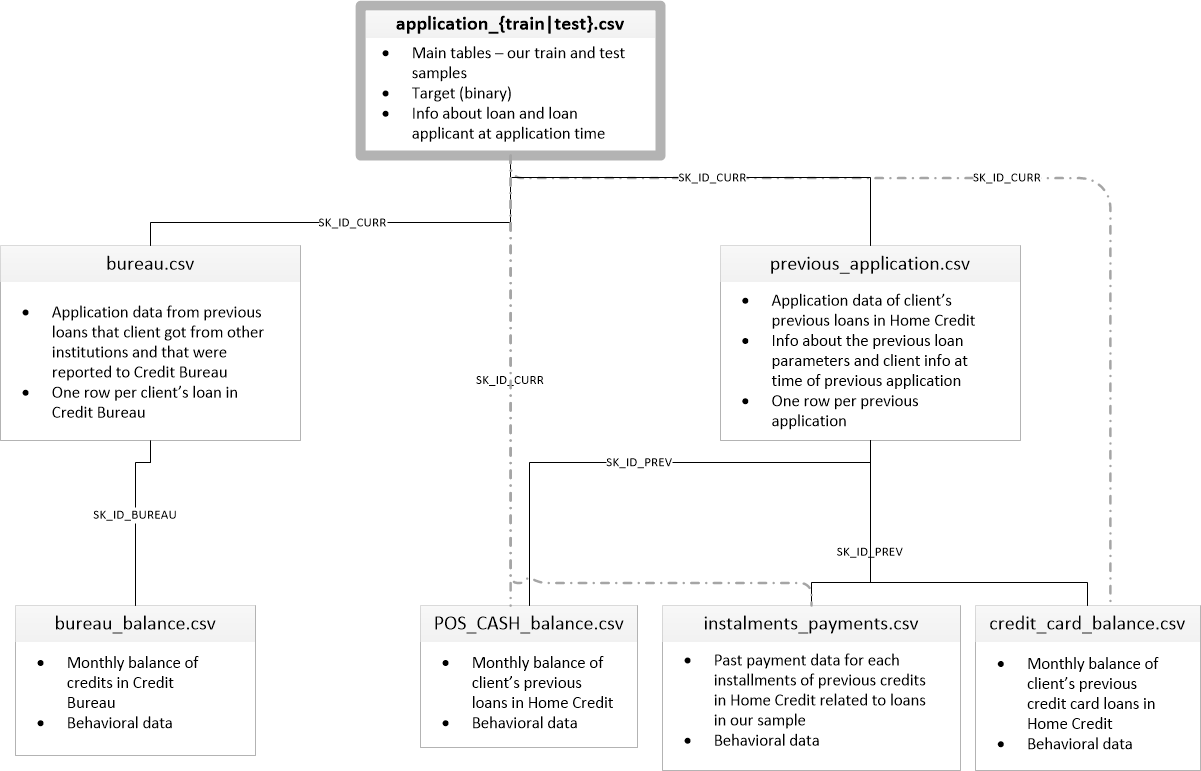
\includegraphics{images/homecredit.png}
\caption{alt text}
\end{figure}

    \begin{Verbatim}[commandchars=\\\{\}]
{\color{incolor}In [{\color{incolor}13}]:} \PY{c+c1}{\PYZsh{} Load the data tables}
         \PY{n}{application\PYZus{}train\PYZus{}data} \PY{o}{=} \PY{n}{pd}\PY{o}{.}\PY{n}{read\PYZus{}csv}\PY{p}{(}\PY{l+s+s2}{\PYZdq{}}\PY{l+s+s2}{data/application\PYZus{}train.csv}\PY{l+s+s2}{\PYZdq{}}\PY{p}{)}
         \PY{n}{application\PYZus{}test\PYZus{}data} \PY{o}{=} \PY{n}{pd}\PY{o}{.}\PY{n}{read\PYZus{}csv}\PY{p}{(}\PY{l+s+s2}{\PYZdq{}}\PY{l+s+s2}{data/application\PYZus{}test.csv}\PY{l+s+s2}{\PYZdq{}}\PY{p}{)}
         \PY{n}{bureau\PYZus{}data} \PY{o}{=} \PY{n}{pd}\PY{o}{.}\PY{n}{read\PYZus{}csv}\PY{p}{(}\PY{l+s+s2}{\PYZdq{}}\PY{l+s+s2}{data/bureau.csv}\PY{l+s+s2}{\PYZdq{}}\PY{p}{)}
         \PY{n}{bureau\PYZus{}balance\PYZus{}data} \PY{o}{=} \PY{n}{pd}\PY{o}{.}\PY{n}{read\PYZus{}csv}\PY{p}{(}\PY{l+s+s2}{\PYZdq{}}\PY{l+s+s2}{data/bureau\PYZus{}balance.csv}\PY{l+s+s2}{\PYZdq{}}\PY{p}{)}
         \PY{n}{previous\PYZus{}application\PYZus{}data} \PY{o}{=} \PY{n}{pd}\PY{o}{.}\PY{n}{read\PYZus{}csv}\PY{p}{(}\PY{l+s+s2}{\PYZdq{}}\PY{l+s+s2}{data/previous\PYZus{}application.csv}\PY{l+s+s2}{\PYZdq{}}\PY{p}{)}
         \PY{n}{POS\PYZus{}CASH\PYZus{}balance\PYZus{}data} \PY{o}{=} \PY{n}{pd}\PY{o}{.}\PY{n}{read\PYZus{}csv}\PY{p}{(}\PY{l+s+s2}{\PYZdq{}}\PY{l+s+s2}{data/POS\PYZus{}CASH\PYZus{}balance.csv}\PY{l+s+s2}{\PYZdq{}}\PY{p}{)}
         \PY{n}{installments\PYZus{}payments\PYZus{}data} \PY{o}{=} \PY{n}{pd}\PY{o}{.}\PY{n}{read\PYZus{}csv}\PY{p}{(}\PY{l+s+s2}{\PYZdq{}}\PY{l+s+s2}{data/installments\PYZus{}payments.csv}\PY{l+s+s2}{\PYZdq{}}\PY{p}{)}
         \PY{n}{credit\PYZus{}card\PYZus{}balance\PYZus{}data} \PY{o}{=} \PY{n}{pd}\PY{o}{.}\PY{n}{read\PYZus{}csv}\PY{p}{(}\PY{l+s+s2}{\PYZdq{}}\PY{l+s+s2}{data/credit\PYZus{}card\PYZus{}balance.csv}\PY{l+s+s2}{\PYZdq{}}\PY{p}{)}
\end{Verbatim}


    \subsubsection{1. Main Data Table
(application\_\{train\textbar{}test\}.csv)}\label{main-data-table-application_traintest.csv}

    \begin{Verbatim}[commandchars=\\\{\}]
{\color{incolor}In [{\color{incolor}14}]:} \PY{c+c1}{\PYZsh{} Display the first five records}
         \PY{n}{display}\PY{p}{(}\PY{n}{application\PYZus{}train\PYZus{}data}\PY{o}{.}\PY{n}{head}\PY{p}{(}\PY{n}{n}\PY{o}{=}\PY{l+m+mi}{5}\PY{p}{)}\PY{p}{)}
\end{Verbatim}


    
    \begin{verbatim}
   SK_ID_CURR  TARGET NAME_CONTRACT_TYPE CODE_GENDER FLAG_OWN_CAR  \
0      100002       1         Cash loans           M            N   
1      100003       0         Cash loans           F            N   
2      100004       0    Revolving loans           M            Y   
3      100006       0         Cash loans           F            N   
4      100007       0         Cash loans           M            N   

  FLAG_OWN_REALTY  CNT_CHILDREN  AMT_INCOME_TOTAL  AMT_CREDIT  AMT_ANNUITY  \
0               Y             0          202500.0    406597.5      24700.5   
1               N             0          270000.0   1293502.5      35698.5   
2               Y             0           67500.0    135000.0       6750.0   
3               Y             0          135000.0    312682.5      29686.5   
4               Y             0          121500.0    513000.0      21865.5   

              ...              FLAG_DOCUMENT_18 FLAG_DOCUMENT_19  \
0             ...                             0                0   
1             ...                             0                0   
2             ...                             0                0   
3             ...                             0                0   
4             ...                             0                0   

  FLAG_DOCUMENT_20 FLAG_DOCUMENT_21 AMT_REQ_CREDIT_BUREAU_HOUR  \
0                0                0                        0.0   
1                0                0                        0.0   
2                0                0                        0.0   
3                0                0                        NaN   
4                0                0                        0.0   

  AMT_REQ_CREDIT_BUREAU_DAY  AMT_REQ_CREDIT_BUREAU_WEEK  \
0                       0.0                         0.0   
1                       0.0                         0.0   
2                       0.0                         0.0   
3                       NaN                         NaN   
4                       0.0                         0.0   

   AMT_REQ_CREDIT_BUREAU_MON  AMT_REQ_CREDIT_BUREAU_QRT  \
0                        0.0                        0.0   
1                        0.0                        0.0   
2                        0.0                        0.0   
3                        NaN                        NaN   
4                        0.0                        0.0   

   AMT_REQ_CREDIT_BUREAU_YEAR  
0                         1.0  
1                         0.0  
2                         0.0  
3                         NaN  
4                         0.0  

[5 rows x 122 columns]
    \end{verbatim}

    
    \begin{Verbatim}[commandchars=\\\{\}]
{\color{incolor}In [{\color{incolor}15}]:} \PY{c+c1}{\PYZsh{} Total number of entries in training group}
         \PY{n+nb}{print}\PY{p}{(}\PY{l+s+s2}{\PYZdq{}}\PY{l+s+s2}{Total number of entries in training group: }\PY{l+s+si}{\PYZob{}\PYZcb{}}\PY{l+s+s2}{\PYZdq{}}\PY{o}{.}\PY{n}{format}\PY{p}{(}\PY{n}{application\PYZus{}train\PYZus{}data}\PY{o}{.}\PY{n}{shape}\PY{p}{[}\PY{l+m+mi}{0}\PY{p}{]}\PY{p}{)}\PY{p}{)}
\end{Verbatim}


    \begin{Verbatim}[commandchars=\\\{\}]
Total number of entries in training group: 307511

    \end{Verbatim}

    \begin{Verbatim}[commandchars=\\\{\}]
{\color{incolor}In [{\color{incolor}16}]:} \PY{c+c1}{\PYZsh{} Total number of entries in test group}
         \PY{n+nb}{print}\PY{p}{(}\PY{l+s+s2}{\PYZdq{}}\PY{l+s+s2}{Total number of entries in test group: }\PY{l+s+si}{\PYZob{}\PYZcb{}}\PY{l+s+s2}{\PYZdq{}}\PY{o}{.}\PY{n}{format}\PY{p}{(}\PY{n}{application\PYZus{}test\PYZus{}data}\PY{o}{.}\PY{n}{shape}\PY{p}{[}\PY{l+m+mi}{0}\PY{p}{]}\PY{p}{)}\PY{p}{)}
\end{Verbatim}


    \begin{Verbatim}[commandchars=\\\{\}]
Total number of entries in test group: 48744

    \end{Verbatim}

    \textbf{Main Data Table Featureset Exploration}

\begin{enumerate}
\def\labelenumi{\arabic{enumi}.}
\tightlist
\item
  \textbf{SK\_ID\_CURR}: ID of loan in our sample
\end{enumerate}

\begin{itemize}
\tightlist
\item
  \textbf{TARGET}: Target variable (1 - client with payment
  difficulties: he/she had late payment more than X days on at least one
  of the first Y installments of the loan in our sample, 0 - all other
  cases)\\
\item
  \textbf{NAME\_CONTRACT\_TYPE}: Identification if loan is cash or
  revolving\\
\item
  \textbf{CODE\_GENDER}: Gender of the client
\item
  \textbf{FLAG\_OWN\_CAR}: Flag if the client owns a car\\
\item
  \textbf{FLAG\_OWN\_REALTY}: Flag if client owns a house or flat\\
\item
  \textbf{CNT\_CHILDREN}: Number of children the client has\\
\item
  \textbf{AMT\_INCOME\_TOTAL}: Income of the client\\
\item
  \textbf{AMT\_CREDIT}: Credit amount of the loan
\item
  \textbf{AMT\_ANNUITY}: Loan annuity
\item
  \textbf{AMT\_GOODS\_PRICE}: For consumer loans it is the price of the
  goods for which the loan is given\\
\item
  \textbf{NAME\_TYPE\_SUITE}: Who was accompanying client when he was
  applying for the loan\\
\item
  \textbf{NAME\_INCOME\_TYPE}: Clients income type (businessman,
  working, maternity leave,Ö)\\
\item
  \textbf{NAME\_EDUCATION\_TYPE}: Level of highest education the client
  achieved
\item
  \textbf{NAME\_FAMILY\_STATUS}: Family status of the client\\
\item
  \textbf{NAME\_HOUSING\_TYPE}: What is the housing situation of the
  client (renting, living with parents, ...)\\
\item
  \textbf{REGION\_POPULATION\_RELATIVE}: Normalized population of region
  where client lives (higher number means the client lives in more
  populated region) -\/- normalized
\item
  \textbf{DAYS\_BIRTH}: Client's age in days at the time of application
  -\/- time only relative to the application
\item
  \textbf{DAYS\_EMPLOYED}: How many days before the application the
  person started current employment -\/- time only relative to the
  application
\item
  \textbf{DAYS\_REGISTRATION}: How many days before the application did
  client change his registration -\/- time only relative to the
  application
\item
  \textbf{DAYS\_ID\_PUBLISH}: How many days before the application did
  client change the identity document with which he applied for the loan
  -\/- time only relative to the application
\item
  \textbf{OWN\_CAR\_AGE}: Age of client's car\\
\item
  \textbf{FLAG\_MOBIL}: Did client provide mobile phone (1=YES, 0=NO)
\item
  \textbf{FLAG\_EMP\_PHONE}: Did client provide work phone (1=YES,
  0=NO)\\
\item
  \textbf{FLAG\_WORK\_PHONE}: Did client provide home phone (1=YES,
  0=NO)\\
\item
  \textbf{FLAG\_CONT\_MOBILE}: Was mobile phone reachable (1=YES,
  0=NO)\\
\item
  \textbf{FLAG\_PHONE}: Did client provide home phone (1=YES, 0=NO)\\
\item
  \textbf{FLAG\_EMAIL}: Did client provide email (1=YES, 0=NO)\\
\item
  \textbf{OCCUPATION\_TYPE}: What kind of occupation does the client
  have
\item
  \textbf{CNT\_FAM\_MEMBERS}: How many family members does client have
\item
  \textbf{REGION\_RATING\_CLIENT}: Our rating of the region where client
  lives (1,2,3)
\item
  \textbf{REGION\_RATING\_CLIENT\_W\_CITY}: Our rating of the region
  where client lives with taking city into account (1,2,3)\\
\item
  \textbf{WEEKDAY\_APPR\_PROCESS\_START}: On which day of the week did
  the client apply for the loan\\
\item
  \textbf{HOUR\_APPR\_PROCESS\_START}: Approximately at what hour did
  the client apply for the loan rounded
\item
  \textbf{REG\_REGION\_NOT\_LIVE\_REGION}: Flag if client's permanent
  address does not match contact address (1=different, 0=same, at region
  level)\\
\item
  \textbf{REG\_REGION\_NOT\_WORK\_REGION}: Flag if client's permanent
  address does not match work address (1=different, 0=same, at region
  level)
\item
  \textbf{LIVE\_REGION\_NOT\_WORK\_REGION}: Flag if client's contact
  address does not match work address (1=different, 0=same, at region
  level)\\
\item
  \textbf{REG\_CITY\_NOT\_LIVE\_CITY}: Flag if client's permanent
  address does not match contact address (1=different, 0=same, at city
  level)\\
\item
  \textbf{REG\_CITY\_NOT\_WORK\_CITY}: Flag if client's permanent
  address does not match work address (1=different, 0=same, at city
  level)\\
\item
  \textbf{LIVE\_CITY\_NOT\_WORK\_CITY}: Flag if client's contact address
  does not match work address (1=different, 0=same, at city level)\\
\item
  \textbf{ORGANIZATION\_TYPE}: Type of organization where client works\\
\item
  \textbf{EXT\_SOURCE\_1}: Normalized score from external data source
  -\/- normalized
\item
  \textbf{EXT\_SOURCE\_2}: Normalized score from external data source
  -\/- normalized
\item
  \textbf{EXT\_SOURCE\_3}: Normalized score from external data source
  -\/- normalized
\item
  \textbf{APARTMENTS\_AVG}: Normalized information about building where
  the client lives, What is average (\_AVG suffix), modus (\_MODE
  suffix), median (\_MEDI suffix) apartment size, common area, living
  area, age of building, number of elevators, number of entrances, state
  of the building, number of floor -\/- normalized
\item
  \textbf{BASEMENTAREA\_AVG}: Normalized information about building
  where the client lives, What is average (\_AVG suffix), modus (\_MODE
  suffix), median (\_MEDI suffix) apartment size, common area, living
  area, age of building, number of elevators, number of entrances, state
  of the building, number of floor -\/- normalized
\item
  \textbf{YEARS\_BEGINEXPLUATATION\_AVG}: Normalized information about
  building where the client lives, What is average (\_AVG suffix), modus
  (\_MODE suffix), median (\_MEDI suffix) apartment size, common area,
  living area, age of building, number of elevators, number of
  entrances, state of the building, number of floor -\/- normalized
\item
  \textbf{YEARS\_BUILD\_AVG}: Normalized information about building
  where the client lives, What is average (\_AVG suffix), modus (\_MODE
  suffix), median (\_MEDI suffix) apartment size, common area, living
  area, age of building, number of elevators, number of entrances, state
  of the building, number of floor -\/- normalized
\item
  \textbf{COMMONAREA\_AVG}: Normalized information about building where
  the client lives, What is average (\_AVG suffix), modus (\_MODE
  suffix), median (\_MEDI suffix) apartment size, common area, living
  area, age of building, number of elevators, number of entrances, state
  of the building, number of floor -\/- normalized
\item
  \textbf{ELEVATORS\_AVG}: Normalized information about building where
  the client lives, What is average (\_AVG suffix), modus (\_MODE
  suffix), median (\_MEDI suffix) apartment size, common area, living
  area, age of building, number of elevators, number of entrances, state
  of the building, number of floor -\/- normalized
\item
  \textbf{ENTRANCES\_AVG}: Normalized information about building where
  the client lives, What is average (\_AVG suffix), modus (\_MODE
  suffix), median (\_MEDI suffix) apartment size, common area, living
  area, age of building, number of elevators, number of entrances, state
  of the building, number of floor -\/- normalized
\item
  \textbf{FLOORSMAX\_AVG}: Normalized information about building where
  the client lives, What is average (\_AVG suffix), modus (\_MODE
  suffix), median (\_MEDI suffix) apartment size, common area, living
  area, age of building, number of elevators, number of entrances, state
  of the building, number of floor -\/- normalized
\item
  \textbf{FLOORSMIN\_AVG}: Normalized information about building where
  the client lives, What is average (\_AVG suffix), modus (\_MODE
  suffix), median (\_MEDI suffix) apartment size, common area, living
  area, age of building, number of elevators, number of entrances, state
  of the building, number of floor -\/- normalized
\item
  \textbf{LANDAREA\_AVG}: Normalized information about building where
  the client lives, What is average (\_AVG suffix), modus (\_MODE
  suffix), median (\_MEDI suffix) apartment size, common area, living
  area, age of building, number of elevators, number of entrances, state
  of the building, number of floor -\/- normalized
\item
  \textbf{LIVINGAPARTMENTS\_AVG}: Normalized information about building
  where the client lives, What is average (\_AVG suffix), modus (\_MODE
  suffix), median (\_MEDI suffix) apartment size, common area, living
  area, age of building, number of elevators, number of entrances, state
  of the building, number of floor -\/- normalized
\item
  \textbf{LIVINGAREA\_AVG}: Normalized information about building where
  the client lives, What is average (\_AVG suffix), modus (\_MODE
  suffix), median (\_MEDI suffix) apartment size, common area, living
  area, age of building, number of elevators, number of entrances, state
  of the building, number of floor -\/- normalized
\item
  \textbf{NONLIVINGAPARTMENTS\_AVG}: Normalized information about
  building where the client lives, What is average (\_AVG suffix), modus
  (\_MODE suffix), median (\_MEDI suffix) apartment size, common area,
  living area, age of building, number of elevators, number of
  entrances, state of the building, number of floor -\/- normalized
\item
  \textbf{NONLIVINGAREA\_AVG}: Normalized information about building
  where the client lives, What is average (\_AVG suffix), modus (\_MODE
  suffix), median (\_MEDI suffix) apartment size, common area, living
  area, age of building, number of elevators, number of entrances, state
  of the building, number of floor -\/- normalized
\item
  \textbf{APARTMENTS\_MODE}: Normalized information about building where
  the client lives, What is average (\_AVG suffix), modus (\_MODE
  suffix), median (\_MEDI suffix) apartment size, common area, living
  area, age of building, number of elevators, number of entrances, state
  of the building, number of floor -\/- normalized
\item
  \textbf{BASEMENTAREA\_MODE}: Normalized information about building
  where the client lives, What is average (\_AVG suffix), modus (\_MODE
  suffix), median (\_MEDI suffix) apartment size, common area, living
  area, age of building, number of elevators, number of entrances, state
  of the building, number of floor -\/- normalized
\item
  \textbf{YEARS\_BEGINEXPLUATATION\_MODE}: Normalized information about
  building where the client lives, What is average (\_AVG suffix), modus
  (\_MODE suffix), median (\_MEDI suffix) apartment size, common area,
  living area, age of building, number of elevators, number of
  entrances, state of the building, number of floor -\/- normalized
\item
  \textbf{YEARS\_BUILD\_MODE}: Normalized information about building
  where the client lives, What is average (\_AVG suffix), modus (\_MODE
  suffix), median (\_MEDI suffix) apartment size, common area, living
  area, age of building, number of elevators, number of entrances, state
  of the building, number of floor -\/- normalized
\item
  \textbf{COMMONAREA\_MODE}: Normalized information about building where
  the client lives, What is average (\_AVG suffix), modus (\_MODE
  suffix), median (\_MEDI suffix) apartment size, common area, living
  area, age of building, number of elevators, number of entrances, state
  of the building, number of floor -\/- normalized
\item
  \textbf{ELEVATORS\_MODE}: Normalized information about building where
  the client lives, What is average (\_AVG suffix), modus (\_MODE
  suffix), median (\_MEDI suffix) apartment size, common area, living
  area, age of building, number of elevators, number of entrances, state
  of the building, number of floor -\/- normalized
\item
  \textbf{ENTRANCES\_MODE}: Normalized information about building where
  the client lives, What is average (\_AVG suffix), modus (\_MODE
  suffix), median (\_MEDI suffix) apartment size, common area, living
  area, age of building, number of elevators, number of entrances, state
  of the building, number of floor -\/- normalized
\item
  \textbf{FLOORSMAX\_MODE}: Normalized information about building where
  the client lives, What is average (\_AVG suffix), modus (\_MODE
  suffix), median (\_MEDI suffix) apartment size, common area, living
  area, age of building, number of elevators, number of entrances, state
  of the building, number of floor -\/- normalized
\item
  \textbf{FLOORSMIN\_MODE}: Normalized information about building where
  the client lives, What is average (\_AVG suffix), modus (\_MODE
  suffix), median (\_MEDI suffix) apartment size, common area, living
  area, age of building, number of elevators, number of entrances, state
  of the building, number of floor -\/- normalized
\item
  \textbf{LANDAREA\_MODE}: Normalized information about building where
  the client lives, What is average (\_AVG suffix), modus (\_MODE
  suffix), median (\_MEDI suffix) apartment size, common area, living
  area, age of building, number of elevators, number of entrances, state
  of the building, number of floor -\/- normalized
\item
  \textbf{LIVINGAPARTMENTS\_MODE}: Normalized information about building
  where the client lives, What is average (\_AVG suffix), modus (\_MODE
  suffix), median (\_MEDI suffix) apartment size, common area, living
  area, age of building, number of elevators, number of entrances, state
  of the building, number of floor -\/- normalized
\item
  \textbf{LIVINGAREA\_MODE}: Normalized information about building where
  the client lives, What is average (\_AVG suffix), modus (\_MODE
  suffix), median (\_MEDI suffix) apartment size, common area, living
  area, age of building, number of elevators, number of entrances, state
  of the building, number of floor -\/- normalized
\item
  \textbf{NONLIVINGAPARTMENTS\_MODE}: Normalized information about
  building where the client lives, What is average (\_AVG suffix), modus
  (\_MODE suffix), median (\_MEDI suffix) apartment size, common area,
  living area, age of building, number of elevators, number of
  entrances, state of the building, number of floor -\/- normalized
\item
  \textbf{NONLIVINGAREA\_MODE}: Normalized information about building
  where the client lives, What is average (\_AVG suffix), modus (\_MODE
  suffix), median (\_MEDI suffix) apartment size, common area, living
  area, age of building, number of elevators, number of entrances, state
  of the building, number of floor -\/- normalized
\item
  \textbf{APARTMENTS\_MEDI}: Normalized information about building where
  the client lives, What is average (\_AVG suffix), modus (\_MODE
  suffix), median (\_MEDI suffix) apartment size, common area, living
  area, age of building, number of elevators, number of entrances, state
  of the building, number of floor -\/- normalized
\item
  \textbf{BASEMENTAREA\_MEDI}: Normalized information about building
  where the client lives, What is average (\_AVG suffix), modus (\_MODE
  suffix), median (\_MEDI suffix) apartment size, common area, living
  area, age of building, number of elevators, number of entrances, state
  of the building, number of floor -\/- normalized
\item
  \textbf{YEARS\_BEGINEXPLUATATION\_MEDI}: Normalized information about
  building where the client lives, What is average (\_AVG suffix), modus
  (\_MODE suffix), median (\_MEDI suffix) apartment size, common area,
  living area, age of building, number of elevators, number of
  entrances, state of the building, number of floor -\/- normalized
\item
  \textbf{YEARS\_BUILD\_MEDI}: Normalized information about building
  where the client lives, What is average (\_AVG suffix), modus (\_MODE
  suffix), median (\_MEDI suffix) apartment size, common area, living
  area, age of building, number of elevators, number of entrances, state
  of the building, number of floor -\/- normalized
\item
  \textbf{COMMONAREA\_MEDI}: Normalized information about building where
  the client lives, What is average (\_AVG suffix), modus (\_MODE
  suffix), median (\_MEDI suffix) apartment size, common area, living
  area, age of building, number of elevators, number of entrances, state
  of the building, number of floor -\/- normalized
\item
  \textbf{ELEVATORS\_MEDI}: Normalized information about building where
  the client lives, What is average (\_AVG suffix), modus (\_MODE
  suffix), median (\_MEDI suffix) apartment size, common area, living
  area, age of building, number of elevators, number of entrances, state
  of the building, number of floor -\/- normalized
\item
  \textbf{ENTRANCES\_MEDI}: Normalized information about building where
  the client lives, What is average (\_AVG suffix), modus (\_MODE
  suffix), median (\_MEDI suffix) apartment size, common area, living
  area, age of building, number of elevators, number of entrances, state
  of the building, number of floor -\/- normalized
\item
  \textbf{FLOORSMAX\_MEDI}: Normalized information about building where
  the client lives, What is average (\_AVG suffix), modus (\_MODE
  suffix), median (\_MEDI suffix) apartment size, common area, living
  area, age of building, number of elevators, number of entrances, state
  of the building, number of floor -\/- normalized
\item
  \textbf{FLOORSMIN\_MEDI}: Normalized information about building where
  the client lives, What is average (\_AVG suffix), modus (\_MODE
  suffix), median (\_MEDI suffix) apartment size, common area, living
  area, age of building, number of elevators, number of entrances, state
  of the building, number of floor -\/- normalized
\item
  \textbf{LANDAREA\_MEDI}: Normalized information about building where
  the client lives, What is average (\_AVG suffix), modus (\_MODE
  suffix), median (\_MEDI suffix) apartment size, common area, living
  area, age of building, number of elevators, number of entrances, state
  of the building, number of floor -\/- normalized
\item
  \textbf{LIVINGAPARTMENTS\_MEDI}: Normalized information about building
  where the client lives, What is average (\_AVG suffix), modus (\_MODE
  suffix), median (\_MEDI suffix) apartment size, common area, living
  area, age of building, number of elevators, number of entrances, state
  of the building, number of floor -\/- normalized
\item
  \textbf{LIVINGAREA\_MEDI}: Normalized information about building where
  the client lives, What is average (\_AVG suffix), modus (\_MODE
  suffix), median (\_MEDI suffix) apartment size, common area, living
  area, age of building, number of elevators, number of entrances, state
  of the building, number of floor -\/- normalized
\item
  \textbf{NONLIVINGAPARTMENTS\_MEDI}: Normalized information about
  building where the client lives, What is average (\_AVG suffix), modus
  (\_MODE suffix), median (\_MEDI suffix) apartment size, common area,
  living area, age of building, number of elevators, number of
  entrances, state of the building, number of floor -\/- normalized
\item
  \textbf{NONLIVINGAREA\_MEDI}: Normalized information about building
  where the client lives, What is average (\_AVG suffix), modus (\_MODE
  suffix), median (\_MEDI suffix) apartment size, common area, living
  area, age of building, number of elevators, number of entrances, state
  of the building, number of floor -\/- normalized
\item
  \textbf{FONDKAPREMONT\_MODE}: Normalized information about building
  where the client lives, What is average (\_AVG suffix), modus (\_MODE
  suffix), median (\_MEDI suffix) apartment size, common area, living
  area, age of building, number of elevators, number of entrances, state
  of the building, number of floor -\/- normalized
\item
  \textbf{HOUSETYPE\_MODE}: Normalized information about building where
  the client lives, What is average (\_AVG suffix), modus (\_MODE
  suffix), median (\_MEDI suffix) apartment size, common area, living
  area, age of building, number of elevators, number of entrances, state
  of the building, number of floor -\/- normalized
\item
  \textbf{TOTALAREA\_MODE}: Normalized information about building where
  the client lives, What is average (\_AVG suffix), modus (\_MODE
  suffix), median (\_MEDI suffix) apartment size, common area, living
  area, age of building, number of elevators, number of entrances, state
  of the building, number of floor -\/- normalized
\item
  \textbf{WALLSMATERIAL\_MODE}: Normalized information about building
  where the client lives, What is average (\_AVG suffix), modus (\_MODE
  suffix), median (\_MEDI suffix) apartment size, common area, living
  area, age of building, number of elevators, number of entrances, state
  of the building, number of floor -\/- normalized
\item
  \textbf{EMERGENCYSTATE\_MODE}: Normalized information about building
  where the client lives, What is average (\_AVG suffix), modus (\_MODE
  suffix), median (\_MEDI suffix) apartment size, common area, living
  area, age of building, number of elevators, number of entrances, state
  of the building, number of floor -\/- normalized
\item
  \textbf{OBS\_30\_CNT\_SOCIAL\_CIRCLE}: How many observation of
  client's social surroundings with observable 30 DPD (days past due)
  default
\item
  \textbf{DEF\_30\_CNT\_SOCIAL\_CIRCLE}: How many observation of
  client's social surroundings defaulted on 30 DPD (days past due)\\
\item
  \textbf{OBS\_60\_CNT\_SOCIAL\_CIRCLE}: How many observation of
  client's social surroundings with observable 60 DPD (days past due)
  default
\item
  \textbf{DEF\_60\_CNT\_SOCIAL\_CIRCLE}: How many observation of
  client's social surroundings defaulted on 60 (days past due) DPD\\
\item
  \textbf{DAYS\_LAST\_PHONE\_CHANGE}: How many days before application
  did client change phone\\
\item
  \textbf{FLAG\_DOCUMENT\_2}: Did client provide document 2\\
\item
  \textbf{FLAG\_DOCUMENT\_3}: Did client provide document 3\\
\item
  \textbf{FLAG\_DOCUMENT\_4}: Did client provide document 4\\
\item
  \textbf{FLAG\_DOCUMENT\_5}: Did client provide document 5\\
\item
  \textbf{FLAG\_DOCUMENT\_6}: Did client provide document 6\\
\item
  \textbf{FLAG\_DOCUMENT\_7}: Did client provide document 7\\
\item
  \textbf{FLAG\_DOCUMENT\_8}: Did client provide document 8\\
\item
  \textbf{FLAG\_DOCUMENT\_9}: Did client provide document 9\\
\item
  \textbf{FLAG\_DOCUMENT\_10}: Did client provide document 10\\
\item
  \textbf{FLAG\_DOCUMENT\_11}: Did client provide document 11\\
\item
  \textbf{FLAG\_DOCUMENT\_12}: Did client provide document 12\\
\item
  \textbf{FLAG\_DOCUMENT\_13}: Did client provide document 13\\
\item
  \textbf{FLAG\_DOCUMENT\_14}: Did client provide document 14\\
\item
  \textbf{FLAG\_DOCUMENT\_15}: Did client provide document 15\\
\item
  \textbf{FLAG\_DOCUMENT\_16}: Did client provide document 16\\
\item
  \textbf{FLAG\_DOCUMENT\_17}: Did client provide document 17\\
\item
  \textbf{FLAG\_DOCUMENT\_18}: Did client provide document 18\\
\item
  \textbf{FLAG\_DOCUMENT\_19}: Did client provide document 19\\
\item
  \textbf{FLAG\_DOCUMENT\_20}: Did client provide document 20\\
\item
  \textbf{FLAG\_DOCUMENT\_21}: Did client provide document 21\\
\item
  \textbf{AMT\_REQ\_CREDIT\_BUREAU\_HOUR}: Number of enquiries to Credit
  Bureau about the client one hour before application
\item
  \textbf{AMT\_REQ\_CREDIT\_BUREAU\_DAY}: Number of enquiries to Credit
  Bureau about the client one day before application (excluding one hour
  before application)\\
\item
  \textbf{AMT\_REQ\_CREDIT\_BUREAU\_WEEK}: Number of enquiries to Credit
  Bureau about the client one week before application (excluding one day
  before application)\\
\item
  \textbf{AMT\_REQ\_CREDIT\_BUREAU\_MON}: Number of enquiries to Credit
  Bureau about the client one month before application (excluding one
  week before application)
\item
  \textbf{AMT\_REQ\_CREDIT\_BUREAU\_QRT}: Number of enquiries to Credit
  Bureau about the client 3 month before application (excluding one
  month before application)\\
\item
  \textbf{AMT\_REQ\_CREDIT\_BUREAU\_YEAR}: Number of enquiries to Credit
  Bureau about the client one day year (excluding last 3 months before
  application)
\end{itemize}

    \subsubsection{2. Bureau Data Table
(bureau\_balance.csv)}\label{bureau-data-table-bureau_balance.csv}

    \begin{Verbatim}[commandchars=\\\{\}]
{\color{incolor}In [{\color{incolor}25}]:} \PY{c+c1}{\PYZsh{} Display the first five records}
         \PY{n}{display}\PY{p}{(}\PY{n}{bureau\PYZus{}data}\PY{o}{.}\PY{n}{head}\PY{p}{(}\PY{n}{n}\PY{o}{=}\PY{l+m+mi}{5}\PY{p}{)}\PY{p}{)}
\end{Verbatim}


    
    \begin{verbatim}
   SK_ID_CURR  SK_ID_BUREAU CREDIT_ACTIVE CREDIT_CURRENCY  DAYS_CREDIT  \
0      215354       5714462        Closed      currency 1         -497   
1      215354       5714463        Active      currency 1         -208   
2      215354       5714464        Active      currency 1         -203   
3      215354       5714465        Active      currency 1         -203   
4      215354       5714466        Active      currency 1         -629   

   CREDIT_DAY_OVERDUE  DAYS_CREDIT_ENDDATE  DAYS_ENDDATE_FACT  \
0                   0               -153.0             -153.0   
1                   0               1075.0                NaN   
2                   0                528.0                NaN   
3                   0                  NaN                NaN   
4                   0               1197.0                NaN   

   AMT_CREDIT_MAX_OVERDUE  CNT_CREDIT_PROLONG  AMT_CREDIT_SUM  \
0                     NaN                   0         91323.0   
1                     NaN                   0        225000.0   
2                     NaN                   0        464323.5   
3                     NaN                   0         90000.0   
4                 77674.5                   0       2700000.0   

   AMT_CREDIT_SUM_DEBT  AMT_CREDIT_SUM_LIMIT  AMT_CREDIT_SUM_OVERDUE  \
0                  0.0                   NaN                     0.0   
1             171342.0                   NaN                     0.0   
2                  NaN                   NaN                     0.0   
3                  NaN                   NaN                     0.0   
4                  NaN                   NaN                     0.0   

       CREDIT_TYPE  DAYS_CREDIT_UPDATE  AMT_ANNUITY  
0  Consumer credit                -131          NaN  
1      Credit card                 -20          NaN  
2  Consumer credit                 -16          NaN  
3      Credit card                 -16          NaN  
4  Consumer credit                 -21          NaN  
    \end{verbatim}

    
    \textbf{Bureau Data Table Featureset Exploration}

\begin{enumerate}
\def\labelenumi{\arabic{enumi}.}
\tightlist
\item
  \textbf{SK\_ID\_CURR}: ID of loan in our sample - one loan in our
  sample can have 0,1,2 or more related previous credits in credit
  bureau -\/- hashed
\end{enumerate}

\begin{itemize}
\tightlist
\item
  \textbf{SK\_BUREAU\_ID}: Recoded ID of previous Credit Bureau credit
  related to our loan (unique coding for each loan application) -\/-
  hashed
\item
  \textbf{CREDIT\_ACTIVE}: Status of the Credit Bureau (CB) reported
  credits\\
\item
  \textbf{CREDIT\_CURRENCY}: Recoded currency of the Credit Bureau
  credit -\/- recoded
\item
  \textbf{DAYS\_CREDIT}: How many days before current application did
  client apply for Credit Bureau credit -\/- time only relative to the
  application
\item
  \textbf{CREDIT\_DAY\_OVERDUE}: Number of days past due on CB credit at
  the time of application for related loan in our sample\\
\item
  \textbf{DAYS\_CREDIT\_ENDDATE}: Remaining duration of CB credit (in
  days) at the time of application in Home Credit -\/- time only
  relative to the application
\item
  \textbf{DAYS\_ENDDATE\_FACT}: Days since CB credit ended at the time
  of application in Home Credit (only for closed credit) -\/- time only
  relative to the application
\item
  \textbf{AMT\_CREDIT\_MAX\_OVERDUE}: Maximal amount overdue on the
  Credit Bureau credit so far (at application date of loan in our
  sample)
\item
  \textbf{CNT\_CREDIT\_PROLONG}: How many times was the Credit Bureau
  credit prolonged
\item
  \textbf{AMT\_CREDIT\_SUM}: Current credit amount for the Credit Bureau
  credit
\item
  \textbf{AMT\_CREDIT\_SUM\_DEBT}: Current debt on Credit Bureau credit
\item
  \textbf{AMT\_CREDIT\_SUM\_LIMIT}: Current credit limit of credit card
  reported in Credit Bureau\\
\item
  \textbf{AMT\_CREDIT\_SUM\_OVERDUE}: Current amount overdue on Credit
  Bureau credit\\
\item
  \textbf{CREDIT\_TYPE}: Type of Credit Bureau credit (Car, cash,...)
\item
  \textbf{DAYS\_CREDIT\_UPDATE}: How many days before loan application
  did last information about the Credit Bureau credit come -\/- time
  only relative to the application
\item
  \textbf{AMT\_ANNUITY}: Annuity of the Credit Bureau credit
\end{itemize}

    \subsubsection{3. Bureau Balance Data Table
(bureau\_balance.csv)}\label{bureau-balance-data-table-bureau_balance.csv}

    \begin{Verbatim}[commandchars=\\\{\}]
{\color{incolor}In [{\color{incolor}24}]:} \PY{c+c1}{\PYZsh{} Display the first five records}
         \PY{n}{display}\PY{p}{(}\PY{n}{bureau\PYZus{}balance\PYZus{}data}\PY{o}{.}\PY{n}{head}\PY{p}{(}\PY{n}{n}\PY{o}{=}\PY{l+m+mi}{5}\PY{p}{)}\PY{p}{)}
\end{Verbatim}


    
    \begin{verbatim}
   SK_ID_BUREAU  MONTHS_BALANCE STATUS
0       5715448               0      C
1       5715448              -1      C
2       5715448              -2      C
3       5715448              -3      C
4       5715448              -4      C
    \end{verbatim}

    
    \textbf{Bureau Balance Data Table Featureset Exploration}

\begin{enumerate}
\def\labelenumi{\arabic{enumi}.}
\tightlist
\item
  \textbf{SK\_BUREAU\_ID}: Recoded ID of Credit Bureau credit (unique
  coding for each application) - use this to join to CREDIT\_BUREAU
  table -\/- hashed
\end{enumerate}

\begin{itemize}
\tightlist
\item
  \textbf{MONTHS\_BALANCE}: Month of balance relative to application
  date (-1 means the freshest balance date) -\/- time only relative to
  the application
\item
  \textbf{STATUS}: Status of Credit Bureau loan during the month
  (active, closed, DPD0-30,Ö {[}C means closed, X means status unknown,
  0 means no DPD, 1 means maximal did during month between 1-30, 2 means
  DPD 31-60,Ö 5 means DPD 120+ or sold or written off {]})
\end{itemize}

    \subsubsection{4. Previous Application Data Table
(previous\_application.csv)}\label{previous-application-data-table-previous_application.csv}

    \begin{Verbatim}[commandchars=\\\{\}]
{\color{incolor}In [{\color{incolor}26}]:} \PY{c+c1}{\PYZsh{} Display the first five records}
         \PY{n}{display}\PY{p}{(}\PY{n}{previous\PYZus{}application\PYZus{}data}\PY{o}{.}\PY{n}{head}\PY{p}{(}\PY{n}{n}\PY{o}{=}\PY{l+m+mi}{5}\PY{p}{)}\PY{p}{)}
\end{Verbatim}


    
    \begin{verbatim}
   SK_ID_PREV  SK_ID_CURR NAME_CONTRACT_TYPE  AMT_ANNUITY  AMT_APPLICATION  \
0     2030495      271877     Consumer loans     1730.430          17145.0   
1     2802425      108129         Cash loans    25188.615         607500.0   
2     2523466      122040         Cash loans    15060.735         112500.0   
3     2819243      176158         Cash loans    47041.335         450000.0   
4     1784265      202054         Cash loans    31924.395         337500.0   

   AMT_CREDIT  AMT_DOWN_PAYMENT  AMT_GOODS_PRICE WEEKDAY_APPR_PROCESS_START  \
0     17145.0               0.0          17145.0                   SATURDAY   
1    679671.0               NaN         607500.0                   THURSDAY   
2    136444.5               NaN         112500.0                    TUESDAY   
3    470790.0               NaN         450000.0                     MONDAY   
4    404055.0               NaN         337500.0                   THURSDAY   

   HOUR_APPR_PROCESS_START            ...            NAME_SELLER_INDUSTRY  \
0                       15            ...                    Connectivity   
1                       11            ...                             XNA   
2                       11            ...                             XNA   
3                        7            ...                             XNA   
4                        9            ...                             XNA   

   CNT_PAYMENT  NAME_YIELD_GROUP       PRODUCT_COMBINATION  \
0         12.0            middle  POS mobile with interest   
1         36.0        low_action          Cash X-Sell: low   
2         12.0              high         Cash X-Sell: high   
3         12.0            middle       Cash X-Sell: middle   
4         24.0              high         Cash Street: high   

   DAYS_FIRST_DRAWING DAYS_FIRST_DUE DAYS_LAST_DUE_1ST_VERSION  DAYS_LAST_DUE  \
0            365243.0          -42.0                     300.0          -42.0   
1            365243.0         -134.0                     916.0       365243.0   
2            365243.0         -271.0                      59.0       365243.0   
3            365243.0         -482.0                    -152.0         -182.0   
4                 NaN            NaN                       NaN            NaN   

  DAYS_TERMINATION NFLAG_INSURED_ON_APPROVAL  
0            -37.0                       0.0  
1         365243.0                       1.0  
2         365243.0                       1.0  
3           -177.0                       1.0  
4              NaN                       NaN  

[5 rows x 37 columns]
    \end{verbatim}

    
    \textbf{Previous Application Data Table Featureset Exploration}

\begin{enumerate}
\def\labelenumi{\arabic{enumi}.}
\tightlist
\item
  \textbf{SK\_ID\_PREV}: ID of previous credit in Home credit related to
  loan in our sample. (One loan in our sample can have 0,1,2 or more
  previous loan applications in Home Credit, previous application could,
  but not necessarily have to lead to credit) -\/- hashed
\end{enumerate}

\begin{itemize}
\tightlist
\item
  \textbf{SK\_ID\_CURR}: ID of loan in our sample -\/- hashed
\item
  \textbf{NAME\_CONTRACT\_TYPE}: Contract product type (Cash loan,
  consumer loan {[}POS{]} ,...) of the previous application\\
\item
  \textbf{AMT\_ANNUITY}: Annuity of previous application\\
\item
  \textbf{AMT\_APPLICATION}: For how much credit did client ask on the
  previous application\\
\item
  \textbf{AMT\_CREDIT}: Final credit amount on the previous application.
  This differs from AMT\_APPLICATION in a way that the AMT\_APPLICATION
  is the amount for which the client initially applied for, but during
  our approval process he could have received different amount -
  AMT\_CREDIT\\
\item
  \textbf{AMT\_DOWN\_PAYMENT}: Down payment on the previous
  application\\
\item
  \textbf{AMT\_GOODS\_PRICE}: Goods price of good that client asked for
  (if applicable) on the previous application\\
\item
  \textbf{WEEKDAY\_APPR\_PROCESS\_START}: On which day of the week did
  the client apply for previous application\\
\item
  \textbf{HOUR\_APPR\_PROCESS\_START}: Approximately at what day hour
  did the client apply for the previous application -\/- rounded
\item
  \textbf{FLAG\_LAST\_APPL\_PER\_CONTRACT}: Flag if it was last
  application for the previous contract. Sometimes by mistake of client
  or our clerk there could be more applications for one single
  contract\\
\item
  \textbf{NFLAG\_LAST\_APPL\_IN\_DAY}: Flag if the application was the
  last application per day of the client. Sometimes clients apply for
  more applications a day. Rarely it could also be error in our system
  that one application is in the database twice\\
\item
  \textbf{RATE\_DOWN\_PAYMENT}: Down payment rate normalized on previous
  credit -\/- normalized
\item
  \textbf{RATE\_INTEREST\_PRIMARY}: Interest rate normalized on previous
  credit -\/- normalized
\item
  \textbf{RATE\_INTEREST\_PRIVILEGED}: Interest rate normalized on
  previous credit -\/- normalized
\item
  \textbf{NAME\_CASH\_LOAN\_PURPOSE}: Purpose of the cash loan\\
\item
  \textbf{NAME\_CONTRACT\_STATUS}: Contract status (approved, cancelled,
  ...) of previous application\\
\item
  \textbf{DAYS\_DECISION}: Relative to current application when was the
  decision about previous application made time only relative to the
  application
\item
  \textbf{NAME\_PAYMENT\_TYPE}: Payment method that client chose to pay
  for the previous application\\
\item
  \textbf{CODE\_REJECT\_REASON}: Why was the previous application
  rejected
\item
  \textbf{NAME\_TYPE\_SUITE}: Who accompanied client when applying for
  the previous application\\
\item
  \textbf{NAME\_CLIENT\_TYPE}: Was the client old or new client when
  applying for the previous application
\item
  \textbf{NAME\_GOODS\_CATEGORY}: What kind of goods did the client
  apply for in the previous application\\
\item
  \textbf{NAME\_PORTFOLIO}: Was the previous application for CASH, POS,
  CAR, Ö
\item
  \textbf{NAME\_PRODUCT\_TYPE}: Was the previous application x-sell o
  walk-in\\
\item
  \textbf{CHANNEL\_TYPE}: Through which channel we acquired the client
  on the previous application\\
\item
  \textbf{SELLERPLACE\_AREA}: Selling area of seller place of the
  previous application\\
\item
  \textbf{NAME\_SELLER\_INDUSTRY}: The industry of the seller\\
\item
  \textbf{CNT\_PAYMENT}: Term of previous credit at application of the
  previous application\\
\item
  \textbf{NAME\_YIELD\_GROUP}: Grouped interest rate into small medium
  and high of the previous application -\/- grouped
\item
  \textbf{PRODUCT\_COMBINATION}: Detailed product combination of the
  previous application
\item
  \textbf{DAYS\_FIRST\_DRAWING}: Relative to application date of current
  application when was the first disbursement of the previous
  application -\/- time only relative to the application
\item
  \textbf{DAYS\_FIRST\_DUE}: Relative to application date of current
  application when was the first due supposed to be of the previous
  application -\/- time only relative to the application
\item
  \textbf{DAYS\_LAST\_DUE\_1ST\_VERSION}: Relative to application date
  of current application when was the first due of the previous
  application -\/- time only relative to the application
\item
  \textbf{DAYS\_LAST\_DUE}: Relative to application date of current
  application when was the last due date of the previous application
  -\/- time only relative to the application
\item
  \textbf{DAYS\_TERMINATION}: Relative to application date of current
  application when was the expected termination of the previous
  application -\/- time only relative to the application
\item
  \textbf{NFLAG\_INSURED\_ON\_APPROVAL}: Did the client requested
  insurance during the previous application
\end{itemize}

    \subsubsection{5. POS CASH Balance Data Table
(POS\_CASH\_balance.csv)}\label{pos-cash-balance-data-table-pos_cash_balance.csv}

    \begin{Verbatim}[commandchars=\\\{\}]
{\color{incolor}In [{\color{incolor}20}]:} \PY{c+c1}{\PYZsh{} Display the first five records}
         \PY{n}{display}\PY{p}{(}\PY{n}{POS\PYZus{}CASH\PYZus{}balance\PYZus{}data}\PY{o}{.}\PY{n}{head}\PY{p}{(}\PY{n}{n}\PY{o}{=}\PY{l+m+mi}{5}\PY{p}{)}\PY{p}{)}
\end{Verbatim}


    
    \begin{verbatim}
   SK_ID_PREV  SK_ID_CURR  MONTHS_BALANCE  CNT_INSTALMENT  \
0     1803195      182943             -31            48.0   
1     1715348      367990             -33            36.0   
2     1784872      397406             -32            12.0   
3     1903291      269225             -35            48.0   
4     2341044      334279             -35            36.0   

   CNT_INSTALMENT_FUTURE NAME_CONTRACT_STATUS  SK_DPD  SK_DPD_DEF  
0                   45.0               Active       0           0  
1                   35.0               Active       0           0  
2                    9.0               Active       0           0  
3                   42.0               Active       0           0  
4                   35.0               Active       0           0  
    \end{verbatim}

    
    \textbf{POS CASH Balance Data Table Featureset Exploration}

\begin{enumerate}
\def\labelenumi{\arabic{enumi}.}
\tightlist
\item
  \textbf{SK\_ID\_PREV}: ID of previous credit in Home Credit related to
  loan in our sample. (One loan in our sample can have 0,1,2 or more
  previous loans in Home Credit)\\
\end{enumerate}

\begin{itemize}
\tightlist
\item
  \textbf{SK\_ID\_CURR}: ID of loan in our sample\\
\item
  \textbf{MONTHS\_BALANCE}: Month of balance relative to application
  date (-1 means the information to the freshest monthly snapshot, 0
  means the information at application - often it will be the same as -1
  as many banks are not updating the information to Credit Bureau
  regularly ) -\/- time only relative to the application
\item
  \textbf{CNT\_INSTALMENT}: Term of previous credit (can change over
  time)\\
\item
  \textbf{CNT\_INSTALMENT\_FUTURE}: Installments left to pay on the
  previous credit\\
\item
  \textbf{NAME\_CONTRACT\_STATUS}: Contract status during the month\\
\item
  \textbf{SK\_DPD}: DPD (days past due) during the month of previous
  credit\\
\item
  \textbf{SK\_DPD\_DEF}: DPD during the month with tolerance (debts with
  low loan amounts are ignored) of the previous credit
\end{itemize}

    \subsubsection{6. Installments Payments Data Table
(installments\_payments.csv)}\label{installments-payments-data-table-installments_payments.csv}

    \begin{Verbatim}[commandchars=\\\{\}]
{\color{incolor}In [{\color{incolor}21}]:} \PY{c+c1}{\PYZsh{} Display the first five records}
         \PY{n}{display}\PY{p}{(}\PY{n}{installments\PYZus{}payments\PYZus{}data}\PY{o}{.}\PY{n}{head}\PY{p}{(}\PY{n}{n}\PY{o}{=}\PY{l+m+mi}{5}\PY{p}{)}\PY{p}{)}
\end{Verbatim}


    
    \begin{verbatim}
   SK_ID_PREV  SK_ID_CURR  NUM_INSTALMENT_VERSION  NUM_INSTALMENT_NUMBER  \
0     1054186      161674                     1.0                      6   
1     1330831      151639                     0.0                     34   
2     2085231      193053                     2.0                      1   
3     2452527      199697                     1.0                      3   
4     2714724      167756                     1.0                      2   

   DAYS_INSTALMENT  DAYS_ENTRY_PAYMENT  AMT_INSTALMENT  AMT_PAYMENT  
0          -1180.0             -1187.0        6948.360     6948.360  
1          -2156.0             -2156.0        1716.525     1716.525  
2            -63.0               -63.0       25425.000    25425.000  
3          -2418.0             -2426.0       24350.130    24350.130  
4          -1383.0             -1366.0        2165.040     2160.585  
    \end{verbatim}

    
    \textbf{Installments Payments Data Table Featureset Exploration}

\begin{enumerate}
\def\labelenumi{\arabic{enumi}.}
\tightlist
\item
  \textbf{SK\_ID\_PREV}: ID of previous credit in Home credit related to
  loan in our sample. (One loan in our sample can have 0,1,2 or more
  previous loans in Home Credit) -\/- hashed
\end{enumerate}

\begin{itemize}
\tightlist
\item
  \textbf{SK\_ID\_CURR}: ID of loan in our sample -\/- hashed
\item
  \textbf{NUM\_INSTALMENT\_VERSION}: Version of installment calendar (0
  is for credit card) of previous credit. Change of installment version
  from month to month signifies that some parameter of payment calendar
  has changed\\
\item
  \textbf{NUM\_INSTALMENT\_NUMBER}: On which installment we observe
  payment\\
\item
  \textbf{DAYS\_INSTALMENT}: When the installment of previous credit was
  supposed to be paid (relative to application date of current loan)
  -\/- time only relative to the application
\item
  \textbf{DAYS\_ENTRY\_PAYMENT}: When was the installments of previous
  credit paid actually (relative to application date of current loan)
  -\/- time only relative to the application
\item
  \textbf{AMT\_INSTALMENT}: What was the prescribed installment amount
  of previous credit on this installment
\item
  \textbf{AMT\_PAYMENT}: What the client actually paid on previous
  credit on this installment
\end{itemize}

    \subsubsection{7. Credit Card Balance Data Table
(credit\_card\_balance.csv)}\label{credit-card-balance-data-table-credit_card_balance.csv}

    \begin{Verbatim}[commandchars=\\\{\}]
{\color{incolor}In [{\color{incolor}22}]:} \PY{c+c1}{\PYZsh{} Display the first five records}
         \PY{n}{display}\PY{p}{(}\PY{n}{credit\PYZus{}card\PYZus{}balance\PYZus{}data}\PY{o}{.}\PY{n}{head}\PY{p}{(}\PY{n}{n}\PY{o}{=}\PY{l+m+mi}{5}\PY{p}{)}\PY{p}{)}
\end{Verbatim}


    
    \begin{verbatim}
   SK_ID_PREV  SK_ID_CURR  MONTHS_BALANCE  AMT_BALANCE  \
0     2562384      378907              -6       56.970   
1     2582071      363914              -1    63975.555   
2     1740877      371185              -7    31815.225   
3     1389973      337855              -4   236572.110   
4     1891521      126868              -1   453919.455   

   AMT_CREDIT_LIMIT_ACTUAL  AMT_DRAWINGS_ATM_CURRENT  AMT_DRAWINGS_CURRENT  \
0                   135000                       0.0                 877.5   
1                    45000                    2250.0                2250.0   
2                   450000                       0.0                   0.0   
3                   225000                    2250.0                2250.0   
4                   450000                       0.0               11547.0   

   AMT_DRAWINGS_OTHER_CURRENT  AMT_DRAWINGS_POS_CURRENT  \
0                         0.0                     877.5   
1                         0.0                       0.0   
2                         0.0                       0.0   
3                         0.0                       0.0   
4                         0.0                   11547.0   

   AMT_INST_MIN_REGULARITY     ...      AMT_RECIVABLE  AMT_TOTAL_RECEIVABLE  \
0                 1700.325     ...              0.000                 0.000   
1                 2250.000     ...          64875.555             64875.555   
2                 2250.000     ...          31460.085             31460.085   
3                11795.760     ...         233048.970            233048.970   
4                22924.890     ...         453919.455            453919.455   

   CNT_DRAWINGS_ATM_CURRENT  CNT_DRAWINGS_CURRENT  CNT_DRAWINGS_OTHER_CURRENT  \
0                       0.0                     1                         0.0   
1                       1.0                     1                         0.0   
2                       0.0                     0                         0.0   
3                       1.0                     1                         0.0   
4                       0.0                     1                         0.0   

   CNT_DRAWINGS_POS_CURRENT  CNT_INSTALMENT_MATURE_CUM  NAME_CONTRACT_STATUS  \
0                       1.0                       35.0                Active   
1                       0.0                       69.0                Active   
2                       0.0                       30.0                Active   
3                       0.0                       10.0                Active   
4                       1.0                      101.0                Active   

   SK_DPD  SK_DPD_DEF  
0       0           0  
1       0           0  
2       0           0  
3       0           0  
4       0           0  

[5 rows x 23 columns]
    \end{verbatim}

    
    \textbf{Credit Card Balance Data Table Featureset Exploration}

\begin{enumerate}
\def\labelenumi{\arabic{enumi}.}
\tightlist
\item
  \textbf{SK\_ID\_PREV}: ID of previous credit in Home credit related to
  loan in our sample. (One loan in our sample can have 0,1,2 or more
  previous loans in Home Credit) -\/- hashed
\end{enumerate}

\begin{itemize}
\tightlist
\item
  \textbf{SK\_ID\_CURR}: ID of loan in our sample -\/- hashed
\item
  \textbf{MONTHS\_BALANCE}: Month of balance relative to application
  date (-1 means the freshest balance date) -\/- time only relative to
  the application
\item
  \textbf{AMT\_BALANCE}: Balance during the month of previous credit\\
\item
  \textbf{AMT\_CREDIT\_LIMIT\_ACTUAL}: Credit card limit during the
  month of the previous credit\\
\item
  \textbf{AMT\_DRAWINGS\_ATM\_CURRENT}: Amount drawing at ATM during the
  month of the previous credit\\
\item
  \textbf{AMT\_DRAWINGS\_CURRENT}: Amount drawing during the month of
  the previous credit\\
\item
  \textbf{AMT\_DRAWINGS\_OTHER\_CURRENT}: Amount of other drawings
  during the month of the previous credit\\
\item
  \textbf{AMT\_DRAWINGS\_POS\_CURRENT}: Amount drawing or buying goods
  during the month of the previous credit\\
\item
  \textbf{AMT\_INST\_MIN\_REGULARITY}: Minimal installment for this
  month of the previous credit\\
\item
  \textbf{AMT\_PAYMENT\_CURRENT}: How much did the client pay during the
  month on the previous credit\\
\item
  \textbf{AMT\_PAYMENT\_TOTAL\_CURRENT}: How much did the client pay
  during the month in total on the previous credit\\
\item
  \textbf{AMT\_RECEIVABLE\_PRINCIPAL}: Amount receivable for principal
  on the previous credit\\
\item
  \textbf{AMT\_RECIVABLE}: Amount receivable on the previous credit\\
\item
  \textbf{AMT\_TOTAL\_RECEIVABLE}: Total amount receivable on the
  previous credit
\item
  \textbf{CNT\_DRAWINGS\_ATM\_CURRENT}: Number of drawings at ATM during
  this month on the previous credit\\
\item
  \textbf{CNT\_DRAWINGS\_CURRENT}: Number of drawings during this month
  on the previous credit
\item
  \textbf{CNT\_DRAWINGS\_OTHER\_CURRENT}: Number of other drawings
  during this month on the previous credit
\item
  \textbf{CNT\_DRAWINGS\_POS\_CURRENT}: Number of drawings for goods
  during this month on the previous credit\\
\item
  \textbf{CNT\_INSTALMENT\_MATURE\_CUM}: Number of paid installments on
  the previous credit
\item
  \textbf{NAME\_CONTRACT\_STATUS}: Contract status (active signed,...)
  on the previous credit\\
\item
  \textbf{SK\_DPD}: DPD (Days past due) during the month on the previous
  credit
\item
  \textbf{SK\_DPD\_DEF}: DPD (Days past due) during the month with
  tolerance (debts with low loan amounts are ignored) of the previous
  credit
\end{itemize}


    % Add a bibliography block to the postdoc
    
    
    
    \end{document}
